% This work is licensed under the Creative Commons
% Attribution-NonCommercial-ShareAlike 4.0 International License. To view a copy
% of this license, visit http://creativecommons.org/licenses/by-nc-sa/4.0/ or
% send a letter to Creative Commons, PO Box 1866, Mountain View, CA 94042, USA.
% vim: set noexpandtab:

\section{Nichtkonforme Methoden} %5
\textbf{Nichtkonform} bedeutet: $V_h\not\subseteq V$\\
\textbf{Konform} bedeutet: $V_h\subseteq V$\\
Warum nichtkonforme Methoden?
\begin{enumerate}[label=(\roman*)]
	\item Probleme höherer Ordnung, z. B. von 4. Ordnung
	\begin{align*}
		V=H^2(\Omega)\qquad\qquad%\\
		\text{Konformität}\implies V_h\subseteq C^1
	\end{align*}
\item Skizze für Zerlegung des Gebietes in vier Teilgebiete, siehe Abbildung \ref{AbbNonconformingMethods}
	\begin{figure}[H]
		\begin{center}
			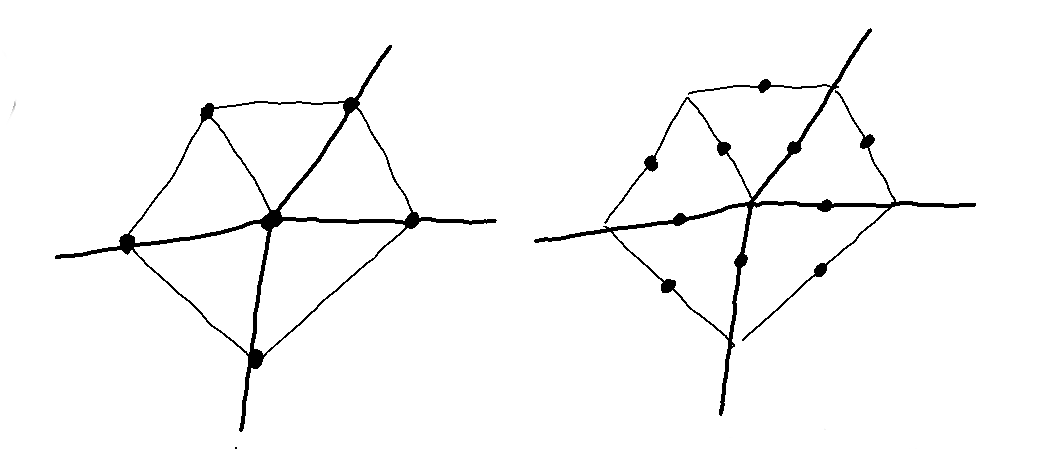
\includegraphics[width=0.75\textwidth]{pics/Sketch5.png}
			\caption{links: konformes $P_1$, rechts nichtkonformes $P_1$}
			\label{AbbNonconformingMethods}
		\end{center}
	\end{figure}
	\item Probleme mit Restriktionen/ Einschränkungen
\end{enumerate}

\subsection{Das nichtkonforme \texorpdfstring{$P_1$}{P\_1}-Element}
Alternative Bezeichnung: Crouzeix-Raviart, 1973\\
Definition lokaler Finite-Elemente $(K,V,\Sigma)$
\begin{align*}
	K&=\text{Dreieck oder Tetraeder}\\
	V&=P_1(K)=\spann\{1,x,y\}\text{ oder }\spann\{1,x,y,z\}\\
	\Sigma&=\big\{N_1,N_2,N_3\big\}\text{ oder }\big\lbrace N_1,N_2,N_3,N_4\big\rbrace\\
	N_i&:\text{ Integral-Mittelwert der Funktionen auf Kanten}\\
	&\text{(äquivalente Alternative: Funktionswerte auf den Mittelpunkten)}
\end{align*}

\begin{beisp}\enter
	\begin{figure}[!ht]
		\begin{center}
			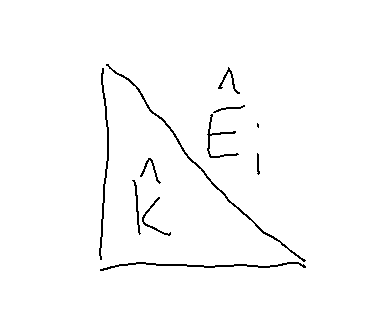
\includegraphics[width=0.25\textwidth]{pics/Sketch6.png}
			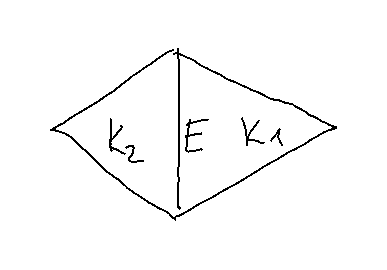
\includegraphics[width=0.25\textwidth]{pics/Sketch7.png}
			\caption{links Referenzdreieck mit Außenkante, rechts Dreiecke mit Innenkante}
			\label{AbbKantentypen}
		\end{center}
	\end{figure}
	\begin{align*}
		\hat{N}_i(\hat{v})=\frac{1}{|\hat{E}_i|}\cdot\int\limits_{\hat{E}_i}\hat{v}\d\gamma
	\end{align*}
\end{beisp}

Der Raum der Finiten-Elemente $V_h$ ist hierbei
\begin{align*}
	V_h=\left\lbrace v\in L^2(\Omega):
	\begin{array}{l}
		v|_K\in P_1(K), \\
		\int\limits_E [v]_E\d\gamma=0~\forall
		\text{ inneren Kanten $E$},\\
		\frac{1}{|E|}\cdot\int\limits_E v\d\gamma=0~\forall\text{ äußeren Kanten }E
	\end{array}
	\right\rbrace
\end{align*}
Hierbei ist $[v]_E$ der Sprung von $v$ über Kanten $E$.\\
\ul{Beobachtung}: Raum der stetigen, stückweise linearen Funktionen ist eine Teilmenge von $V_h$ mit Nullrandbedingungen (d.h. die Funktionen verschwinden auf dem Rand). Es folgt
\begin{align*}
	\inf\limits_{v_h\in V_h}\big\Vert u-v_h\big\Vert_{0,2,\Omega}
	\leq\inf\limits_{w_h\in S_{h,0}^{1,0}}\big\Vert u-w_h\big\Vert_{0,2,\Omega}
	\leq c\cdot h^2\cdot|u|_{2,2,\Omega}
\end{align*}
Wegen $V_h\not\subseteq V$ brauchen wir die Verallgemeinerung von $|\cdot|_{1,2,\Omega}$ für $v\in V=H^1_0(\Omega)$:
\begin{align*}
	|v|_{1,2,\Omega}^2
	&=\sum\limits_{K\in\T_h}|v|^2_{1,2,K}
	=\sum\limits_{K\in\T_h}\Big| v|_K\Big|^2_{1,2,K}
\end{align*}
Definiere
\begin{align*}
	|v|_{1,h}:=\left(\sum\limits_{K\in\T_h}|v|^2_{1,2,K}\right)^{\frac{1}{2}}
\end{align*}
Ist $|\cdot|_{1,h}$ eine Norm auf $V_h$? Es reicht die Null-Eigenschaft zu prüfen:
\begin{align*}
	|v_{1,h}|=0\implies v|_K=\text{konst.}
	\stackrel{\int\limits_E[v]_E\d\gamma=0}{\implies}
	v=\text{konst. auf }\Omega
	\stackrel{\int\limits_{E\in\Gamma} v\d\gamma=0}{\implies}
	v\equiv 0
\end{align*}
Folglich ist es wirklich eine Norm. Es gilt außerdem:
\begin{align*}
	\inf\limits_{v_h\in V_h}\big|u-v_h\big|_{1,h}
	\leq\inf\limits_{w_h\in S_{h,0}^{1,0}}\underbrace{\big|u-w_h\big|_{1,h}}_{|u-w_h|_{1,2}}
	\leq c\cdot h\cdot|u|_{2,2}
\end{align*}

\subsection{Abstraktes Framework}
Wir betrachten unser Modellproblem:
\begin{align*}
	\left\lbrace\begin{array}{rl}
		-\Delta u=f&\text{ in }\Omega\\
		u=0& \text{ auf }\Gamma=\partial\Omega
	\end{array}\right.
\end{align*}
Variationsformulierung: Finde $u\in V=H_0^1(\Omega)$ so, dass
\begin{align*}
	\underbrace{\int\limits_\Omega\nabla u\cdot\nabla v\d x}_{=:a(u,v)}=\underbrace{\int\limits_\Omega f\cdot v\d x}_{=:(f,v)}\qquad\forall v\in V
\end{align*}
Schwierigkeit: $a$ ist nicht definiert für alle Funktionen aus $V_h$. Setze
\begin{align*}
	a_h(v_h,w_h):=\sum\limits_{K\in\mathcal{T}_h}\int\limits_K\nabla v_h\cdot\underbrace{\nabla w_h}_{=\nabla(w_h|_K)}\d x
\end{align*}
Diskretes Problem: Finde $u_h\in V_h$ so, dass
\begin{align*}
	a_h(u_h,v_h)=(f,v_h)\qquad\forall v_h\in V_h
\end{align*}

\textbf{Annahmen:}
\begin{itemize}
	\item $V$ sei ein Hilbertraum
	\item $V_h$ sei ein diskreter Finite-Elemente-Raum mit Norm $\Vert\cdot\Vert_h$
	\item $a\colon V\times V\to\R$ sei ein stetige, $V$-elliptische Bilinearform
	\item $f\colon V\to\R$ sei linear und stetig
\end{itemize}
Dann sagt Lax-Milgram \ref{theorem2.1LaxMilgram}: Es existiert genau ein $u\in V$, welches das Problem löst.\nl
\textbf{Weitere Annahmen:}
\begin{itemize}
	\item $a_h$ sei eine Bilinearform auf $V+ V_h:=\big\lbrace v+v_h: v\in V,v_h\in V_h\big\rbrace$
	\item $a_h$ sei \textbf{gleichmäßig stetig auf $V+ V_h$}, d. h.
	\begin{align*}
		\exists M>0\text{ unabhängig von }h:\big|a_h(u,v)\big|\leq M\cdot\Vert u\Vert_h\cdot\Vert v\Vert_h\qquad\forall u,v\in V+ V_h
	\end{align*}
	\item $f_h\colon V_h + V\to\R$ sei linear und stetig % orig: \cup, aber warum, wir haben doch überall + ?!
	\item $a_h$ ist \textbf{gleichmäßig $V_h$-elliptisch}, d.h.
	\begin{align*}
		\alpha\cdot\Vert v_h\Vert^2_h\leq a_h(v_h,v_h)\qquad\forall v_h\in V_h
	\end{align*}
	wobei $\alpha$ unabhängig von $v_h$ und $h$ ist.
\end{itemize}
Dann sagt Lax-Milgram \ref{theorem2.1LaxMilgram}: Es existiert genau ein $u_h\in V_h$, welches das Problem löst. Welcher Zusammenhang besteht nun zwischen $u$ und $u_h$?

\begin{theorem}[Zweites Lemma von Strang]\label{theorem5.1ZweitesLemmaStrang}\enter
	Sei $\lbrace V_h\rbrace$ eine Familie von (nichtkonformen) Finiten-Elementen-Räumen. Bezeichne $u$ und $u_h$ die schwache bzw. die diskrete Lösung. Dann gilt:
	\begin{align*}
		\big\Vert u-u_h\big\Vert_h\leq\left(1+\frac{M}{\alpha}\right)\cdot\inf\limits_{v_h\in V_h}\big\Vert u-v_h\big\Vert_h
		+\frac{1}{\alpha}\cdot\sup\limits_{z_h\in V_h}\frac{a_h(u,z_h)-f_h(z_h)}{\Vert z_h\Vert_h}
	\end{align*}
	Hierbei ist erste Summand auf der rechten Seite der Approximationsfehler und der zweite Term der Konsistenzfehler.
\end{theorem}

\begin{bemerkung}
	konforme Methode: $V_h\subseteq V,~a_h=a,f_h=f$ und damit:
	\begin{align*}
		a_h(u,z_h)-f_h(z_h)=a(u_h,z_h)-f(z_h)=0\text{ wegen } z_h\in V_h\subseteq V
	\end{align*}
	Folglich gibt es im Fall der konformen Methode keinen Konsistenzfehler.
\end{bemerkung}

\begin{proof}
	Sei $v_h\in V_h$ beliebig, $w_h\coloneqq v_h-u_h$. Dann gilt:
	\begin{align*}
		α \norm{v_h-u_h}_h^2
		&\leq a_h\big(v_h-u_h,v_h-u_h\big) = a_h\big(v_h-u_h, w_h\big)\\
		&=a_h\big(v_h,w_h\big)-\underbrace{a_h\big(u_h,w_h\big)}_{=f_h(w_h)}\\
		&=a_h\big(v_h-u,w_h\big)+a_h\big(u,w_h\big)-f_h\big(w_h\big)\cdot\frac{\Vert w_h\Vert_h}{\Vert w_h\Vert_h}\\
		&\leq M\cdot\big\Vert v_h-u\big\Vert_h\cdot\big\Vert w_h\big\Vert_h+\Vert w_h\Vert_h\cdot\sup\limits_{z_h\in V_h}\frac{a_h\big(u,z_h\big)-f_h\big(z_h\big)}{\Vert z_h\Vert_h}\\
		\implies
		\underbrace{\norm{w_h}_h}_{=\norm{v_h-u_h}_h}
		&\leq\frac M{α} · \norm{v_h-u}_h
		+ \frac1{α} · \sup_{z_h ∈ V_h} \frac{a_h\big(u,z_h\big)-f_h\big(z_h\big)}{\norm{z_h}_h}
	\end{align*}
	Mit der Dreicksungleichung folgt:
	\begin{align*}
		\norm{u-u_h}_h
		&\leq \norm{u-v_h}_h + \norm{v_h-u_h}_h\\
		&\leq\left(1+\frac{M}{\alpha}\right)\cdot\Vert u-v_h\Vert_h+\frac{1}{\alpha}\cdot\sup\limits_{z_h\in V_h}\frac{a_h\big(u,z_h\big)-f_h\big(z_h\big)}{\Vert z_h\Vert_h}
	\end{align*}
	Bilden des Infimums $\inf\limits_{v_h\in V_h}$ liefert die Behauptung.
\end{proof}

\subsection{Überprüfen der Voraussetzungen für das Poisson-Problem}
\begin{align*}
	a_h(v_h,w_h)&=\sum\limits_{K\in\T_h}\int\limits_K\nabla v_h\cdot\nabla w_h\d x\\
	f_h(v_h)&=\sum\limits_{K\in\T_h}\int\limits_K f\cdot v_h\d x\\
	\Vert v\Vert_h&=\left(\sum\limits_{K\in\T_h}|v|_{1,2,K}\right)^{\frac{1}{2}}
\end{align*}
$\Vert\cdot\Vert_h$ ist eine Norm auf $V+ V_h$.\\
Gleichmäßige Stetigkeit von $a_h$ auf $V+ V_h$: Seien $v,w\in V\cup V_h$. Dann gilt:
\begin{align*}
	\big|a_h(v,w)\big|
	&=\left|\sum\limits_{K\in\T_h}\int\limits_K\nabla v\cdot\nabla w\d x\right|\\
	\overset{\text{CS}}&\leq
	\sum\limits_{K\in\T_h}|v|_{1,2,K}\cdot |w|_{1,2,K}\\
	\overset{\text{CS}}&\leq
	\left(\sum\limits_{K\in\T_h} |v|_{1,2,K}^2\right)^{\frac{1}{2}}\cdot\left(\sum\limits_{K\in\T_h}|w|_{1,2,K}^2\right)^{\frac{1}{2}}\\
	&=\Vert v\Vert_h\cdot\Vert w\Vert_h \quad
	(\implies M=1)
\end{align*}
Gleichmäßige $V_h$-Elliptizität von $a_h$ auf $V_h$: Sei $v_h\in V_h$ beliebig. Dann gilt:
\begin{align*}
	a_h(v_h,v_h)
	&=\sum\limits_{K\in\T_h}\int\limits_K\nabla v_h\cdot\nabla v_h\d x
	=\sum\limits_{K\in\T_h}|v_h|^2_{1,2,K}
	=\Vert v_h\Vert^2_h \quad
	(\implies\alpha=1)
\end{align*}
Stetigkeit von $f_h$ auf $V_h$:
\begin{align*}
	\big|f_h(v_h)\big|
	&=\left|\sum\limits_{K\in\T_h}\int\limits_K f\cdot v_h\d x\right|
	\overset{\text{}}\leq
	\sum\limits_{K\in\T_h}\Vert f \Vert_{0,2,K}\cdot\Vert v_h\Vert_{0,2,K}
	\overset{\text{}}\leq
	\Vert f\Vert_{0,2,\Omega}\cdot\Vert v_h\Vert_{0,2,\Omega}
\end{align*}
Auf $V_h$ (endlich-dimensionaler Raum) sind die Normen $\Vert\cdot\Vert_h$ und $\Vert\cdot\Vert_{0,2,\Omega}$ äquivalent:
\begin{align*}
	\implies
	\big|f_h(v_h)\big|
	\leq
	c_h\cdot\Vert f\Vert_{0,2,\Omega}\cdot\Vert v_h\Vert_h
\end{align*}

\subsection{Fehlerabschätzung} %5.4
Bisher:
\begin{align*}
	\Vert u-u_h\Vert_h
	&\leq
	2\cdot\underbrace{\inf\limits_{v_h\in V_h}\Vert u-v_h\Vert_h}_{\leq c\cdot h\cdot |u|_{2,2}}+1\cdot\underbrace{\sup\limits_{z_h\in V_h}\frac{a_h(u,z_h)-f_h(z_h)}{\Vert z_h\Vert_h}}_{\leq?}
\end{align*}
Sei $f\in L^2(\Omega)$ und $u\in H^2(\Omega)$. Dann:
\begin{align*}
	-\laplace u=f \text{ im $L^2$-Sinn auf jedem } K ∈ \T_h
\end{align*}
Sei nun $z_h\in V_h$ beliebig. Dann gilt:
\begin{align*}
	Σ_{K∈\T_h}∫\limits_K-\laplace u · z_h\d x
	&=Σ_{K∈\T_h}∫\limits_K f · z_h\d x\\
	Σ_{K∈\T_h}∫\limits_K-\laplace u · z_h\d x
	\overset{\text{part. Int.}}&=
	Σ_{K∈\T_h}\left(∫\limits_K∇ u · ∇ z_h\d x-∫\limits_{\Rand K}\underbrace{\frac{∂ u}{∂ n_K}}_{=∇ u · n_K}z_h\d γ \right)\\
	\implies L_h(z_h)
	&\coloneqq a_h(u,z_h)-f_h(z_h)\\
	&=Σ_{K∈\T_h}∫\limits_{\Rand K}\frac{∂ u}{∂ n_K}z_h\d γ \\
	&=Σ_{E}∫\limits_E\underbrace{\left[\frac{∂ u}{∂ u_E}z_h\right]_E}_{=\frac{∂ u}{∂ u_E}[z_h]_E}\d γ \\
	&=Σ_E∫\limits_E\frac{∂ u}{∂ u_E}[z_h]_E\d γ \\
	\text{wobei } [v]_E &\coloneqq v|_{K_1}-v|_{K_2}
\end{align*}
\begin{figure}[!ht]
	\begin{center}
		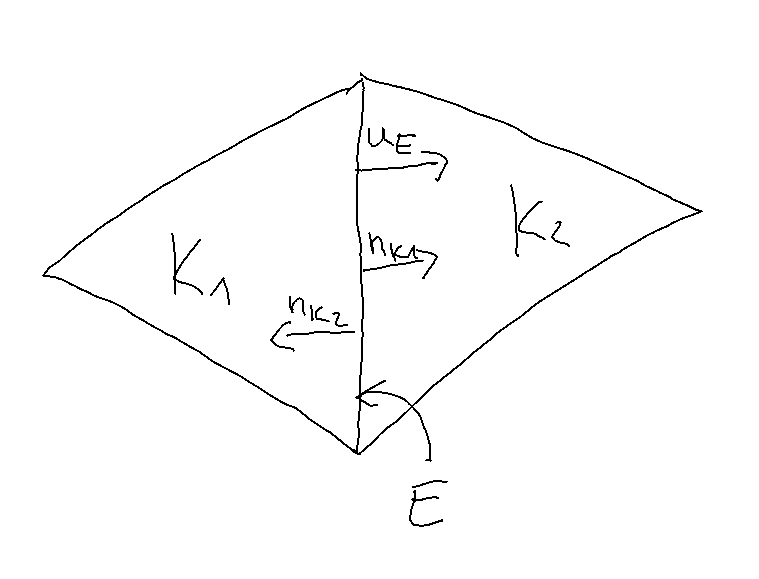
\includegraphics[width=0.75\textwidth]{pics/Sketch8.png}
		\caption{Skizze der Normalen an Kante zwischen zwei Dreiecken}
		\label{AbbNormalvectors}
	\end{center}
\end{figure}
Seien $\overline{z}_h$ und $\overline{\frac{\partial u}{\partial u_E}}$ die konstanten Integral-Mittelwerte von $z_h$ und $\frac{\partial u}{\partial u_E}$ auf jedem $E$, formal:
\begin{align*}
	\overline{z}_h|_E
	:&=\frac{1}{|E|}\cdot\int\limits_E z_h\d\gamma,\qquad\left.\overline{\frac{\partial u}{\partial u_E}}\right|_E \coloneqq \frac{1}{|E|}\cdot\int\limits_E \frac{\partial u}{\partial u_E}\d\gamma
\end{align*}
Mit
\begin{align*}
	\int\limits_E[z_h]_E\d\gamma=0\text{ wegen }z_h\in V_h
\end{align*}
und da $\overline{\frac{\partial u}{\partial u_E}}$ eine Konstante ist
folgt
\begin{align*}
	\int\limits_E\frac{\partial u}{\partial u_E}[z_h]_E\d\gamma
	&=\int\limits_E\left(\frac{\partial u}{\partial u_E}-\overline{\frac{\partial u}{\partial u_E}}\right)[z_h]_E\d\gamma
	=\int\limits_E\left(\frac{\partial u}{\partial u_E}-\overline{\frac{\partial u}{\partial u_E}}\right)[z_h-\overline{z}_h]_E\d\gamma\\
	\implies
	L_h(z_h)
	&=\sum\limits_{K\in\T_h}\sum\limits_{E\subseteq\partial K}\int\limits_E\left(\frac{\partial u}{\partial u_E}-\overline{\frac{\partial u}{\partial u_E}}\right)\big[z_h-\overline{z}_h\big]_E\d\gamma\\
	\overset{\text{CS}}&\leq
	\sum\limits_{K\in\T_h}\sum\limits_{E\subseteq\partial K}\left\Vert\frac{\partial u}{\partial u_E}-\overline{\frac{\partial u}{\partial u_E}}\right\Vert_{0,2,E}\cdot\Vert z_h-\overline{z}_h\Vert_{0,2,E}
\end{align*}
Berechne nun für die Differenz: $z_h-\overline{z}_h$:
\begin{align*}
	\big\Vert z_h-\overline{z}_h\big\Vert_{0,2,E}
	&\leq
	c\cdot\underbrace{\big\Vert B_E^{-1}\big\Vert^0}_{=1}\cdot{\underbrace{\big|\det(B_E)\big|}_{=h_E}}^{\frac{1}{2}}\cdot\big\Vert \underbrace{\hat{z}_h-		\hat{\overline{z}}_h}_{=\widehat{z_h-\overline{z}_h}}\big\Vert_{0,2,\hat{E}}\\
	&\leq
	c\cdot h_E^{\frac{1}{2}}\cdot\big\Vert\widehat{z_h-\overline{z}_h}\big\Vert_{0,2,\hat{E}}
\end{align*}
Der Operator
\begin{align*}
	L\colon H^1(\hat{K})\to L_2(\hat{E}),\qquad\hat{v}\mapsto\left(\hat{v}-\overline{\hat{v}}\right)|_{\hat{E}}
	\mit \overline{\hat{v}}=\frac{1}{|\hat{E}|}\cdot\int\limits_{\hat{E}}\hat{v}\d\gamma
\end{align*}
ist linear und stetig. Folglich gilt:
\begin{align*}
	\big\Vert L(\hat{v})\big\Vert_{0,2,\hat{E}}
	&=\big\Vert\hat{v}-\overline{\hat{v}}\big\Vert_{0,2,\hat{E}}
	\leq
	\underbrace{\Vert\hat{v}\Vert_{0,2,\hat{E}}}_{\stackrel{\text{Spursatz}}{\leq} c\cdot\Vert\hat{v}\Vert_{1,2,\hat{K}}}+\big\Vert\overline{\hat{v}}\big		\Vert_{0,2,\hat{E}}\\
	\big\Vert\overline{\hat{v}}\big\Vert^2_{0,2,\hat{E}}
	&=
	\int\limits_{\hat{E}}\big|\overline{\hat{v}}\big|^2\d\gamma \\
	&=
	\left(\frac{1}{|\hat{E}|}\cdot\int\limits_{\hat{E}}\hat{v}\d\gamma\right)^2\cdot|\hat{E}|\\
	&\leq
	\frac{1}{|\hat{E}|^2}\cdot\Big(\underbrace{\Vert1\Vert_{0,2,\hat{E}}}_{=|\hat{E}|^{\frac{1}{2}}}\cdot\Vert\hat{v}\Vert_{0,2,\hat{E}}\Big)^2\cdot|\hat{E}|\\
	&=\Vert\hat{v}\Vert^2_{0,2,\hat{E}}\\
	&\leq c\cdot\Vert\hat{v}\Vert_{1,2,\hat{K}}
\end{align*}
Somit:
\begin{align*}
	\implies
	\big\Vert L(\hat{v})\big\Vert_{0,2,\hat{E}}
	&\leq c\cdot\Vert\hat{v}\Vert_{1,2,\hat{K}}
\end{align*}
Außerdem
\begin{align*}
	%\implies
	L(\hat{w})&=0\qquad\forall\hat{w}\in P_0(\hat{K})\\
	\overset{\text{Bramble-Hilbert}}{\implies}
	\big\Vert L(\hat{v})\big\Vert_{0,2,\hat{E}}
	&\leq
	c\cdot|\hat{v}|_{1,2,\hat{K}}\\
	\implies
	\big\Vert z_h-\overline{z}_h\big\Vert_{0,2,E}
	&\leq c\cdot h_E^{\frac{1}{2}}\cdot\big|\hat{z}_h\big|_{1,2,\hat{K}}\\
	\overset{\text{transf. zurück}}&{\leq}
	c\cdot h_E^{\frac{1}{2}}\cdot\underbrace{\Vert B_K\Vert^1}_{\sim h_K}\cdot{\underbrace{\big|\det(B_K)\big|}_{\sim h_K^2}}^{-\frac{1}{2}}\cdot|z_h|_{1,2,K}\\
	&\leq
	c\cdot h_E^{\frac{1}{2}}\cdot|z_h|_{1,2,K}
\end{align*}
Auf ähnliche Art und Weise, aber mit wesentlich mehr Aufwand, erhält man auch:
\begin{align*}
	\left\Vert\frac{\partial u}{\partial u_K}-\overline{\frac{\partial u}{\partial u_K}}\right\Vert_{0,2,E}
	&\leq c\cdot h_E^{\frac{1}{2}}\cdot\Vert u\Vert_{2,2,K}
\end{align*}
Nun können wir endlich alle Abschätzungen zusammenbringen und erhalten
\begin{align*}
	\implies
	L_h(z_h)
	&\leq
	\sum\limits_{K\in\T_h}\sum\limits_{E\subseteq\partial K}\left\Vert\frac{\partial u}{\partial u_K}-\overline{\frac{\partial u}{\partial u_K}}\right\Vert_{0,2,E}\cdot\big\Vert z_h-\overline{z}_h\big\Vert_{0,2,E}\\
	&\leq
	c\cdot\sum\limits_{K\in\T_h} h^{\frac{1}{2}}\cdot\Vert u\Vert_{2,2,K}\cdot h^{\frac{1}{2}}\cdot|z_h|_{1,2,K}\\
	&\leq
	c\cdot h\cdot\left(\sum\limits_{K\in\T_h}\Vert u\Vert^2_{1,2,K}\right)^{\frac{1}{2}}\cdot\left(\sum\limits_{K\in\T_h}|z_h|_{1,2,K}^2\right)^{\frac{1}{2}}\\
	&=c\cdot h\cdot \Vert u\Vert_{2,2,\Omega}\cdot\Vert z_h\Vert_h\\
	\implies
	\sup\limits_{z_h\in V_h}\frac{a_h(u, z_h)-f_h(z_h)}{\Vert z_h\Vert_h}
	&\leq c\cdot h\cdot\Vert u\Vert_{2,2,\Omega}
\end{align*}

\begin{theorem}\label{theorem5.2}
	Sei $\lbrace V_h\rbrace$ eine Familie von $P_1$-nichtkonformen Finite-Elemente-Räume, wobei $u_h\in V_h$ das diskrete Problem löst und $u\in V\cap H^2(\Omega)$ die Lösung der schwachen Formulierung ist. Dann gilt:
	\begin{align*}
		\big\Vert u-u_h\big\Vert_h\leq c\cdot h\cdot\Vert u\Vert_{2,2,\Omega}
	\end{align*}
\end{theorem}

\begin{bemerkung}
	Das Dualitätsargument von Aubin und Nietsche kann erweitert werden auf den nichtkonformen Fall. Dabei tauchen zwei neue Terme in der Abschätzung auf.
	\begin{align*}
		\big\Vert u-u_h\big\Vert_{0,2,\Omega}\leq c\cdot h^2\cdot\Vert u\Vert_{2,2,\Omega}
	\end{align*}
\end{bemerkung}